\documentclass[journal]{IEEEtran}
\usepackage[utf8]{inputenc}

\usepackage{hyperref}
\usepackage{graphicx}
\ifCLASSINFOpdf
\else
\fi
\usepackage{amsfonts}
\usepackage{color}
%\usepackage[dvipsnames]{xcolor}
\usepackage{soul}
\hyphenation{op-tical net-works semi-conduc-tor ns- however}
\usepackage{subcaption}
\usepackage{tabularx,booktabs}
\usepackage{amsmath,amssymb,amsfonts}
\usepackage{textcomp}
\usepackage{url}
\usepackage{multirow}
\newcommand{\cmark}{\ding{51}}%
\newcommand{\xmark}{\ding{55}}%
\usepackage[table,xcdraw]{xcolor}

\usepackage{boldline}
\usepackage{amssymb}
\usepackage{pifont}

\usepackage[noadjust]{cite}
\renewcommand{\citepunct}{,\penalty\citepunctpenalty\,}
\renewcommand{\citedash}{--}% optionally

\begin{document}
	\title{Usage of Network Simulators in \\Machine-Learning-Assisted 5G/6G Networks}
	
	\author{Francesc~Wilhelmi,~Marc~Carrascosa,~Cristina~Cano,~Anders~Jonsson,~Vishnu~Ram,~and~Boris~Bellalta%
		\thanks{Francesc Wilhelmi, Marc Carrascosa, Anders Jonsson, and Boris Bellalta are with Universitat Pompeu Fabra (UPF); Cristina Cano is with Universitat Oberta de Catalunya (UOC)); Vishnu Ram is currently working as an independent researcher.}% <-this % stops a space
	}
	
	\maketitle
	
	\begin{abstract}
		Without any doubt, Machine Learning (ML) will be an important driver of future communications due to its foreseen performance in front of complex problems. However, the application of ML to networking systems raises concerns among network operators and other stakeholders, especially regarding trustworthiness and reliability. In this paper, we devise the role of network simulators for bridging the gap between ML and communications systems. Network simulators can facilitate the adoption of ML-based solutions by means of training, testing, and validating ML models before being applied to an operative network. Finally, we showcase the potential benefits of integrating network simulators into ML-assisted communications through a proof-of-concept testbed implementation of a residential Wi-Fi network. 
	\end{abstract}
	
	\begin{IEEEkeywords}
		Future Networks, ITU, Network Simulator, Machine Learning, Wireless Local Area Networks
	\end{IEEEkeywords}
	
	\IEEEpeerreviewmaketitle
	
	\section{Introduction}
	Beyond the fifth-generation (5G) of mobile communications systems, namely the sixth generation (6G), Artificial Intelligence (AI), and more precisely Machine Learning (ML), are expected to be pervasively included as part of the network operation, which would entail a huge leap towards optimization, automation, and self-healing. This is possible thanks to the paradigm shift driven by the softwarization of networks -- achieved through Software Defined Networks (SDN) and Network Function Virtualization (NFV) -- which provides the necessary flexibility to empower data-driven approaches.
	
	The integration of ML to communications has started to be considered for the upcoming versions of 5G. This fact is supported by the content already approved by the 3rd Generation Partnership Project (3GPP) for Release 16 (2020) and Release 17 (2021) \cite{3gpp2019study}, which aim to continue improving the efficiency of 5G systems in many domains such as interference mitigation, Self-Organizing Networks (SON) and Big Data, power consumption, and user mobility, to name a few. Besides, we find of high relevance the contributions made by the International Telecommunication Union (ITU) Focus Group on Machine Learning for 5G and Beyond (FG-ML5G) and the Study Group 13 (SG13), which have published specifications on an ML-aware architecture \cite{ITU3172, ITU3174}.
	
	Through the exploitation of the rich amount of available data, ML can overcome the systemic complexity inherited from novel use cases like Vehicle to Everything (V2X) communications, Machine Type Communications (mMTC), and extended reality and high-quality video content delivery. These use cases comprise heterogeneous scenarios with mobility, a huge number of devices, and high-bandwidth and low-latency requirements. In particular, ML may offer substantial performance gains due to the inherent flexibility of automatically learning diverse situations, thus allowing to solve problems related to interference management, improving spatial reuse, or efficient resource allocation.
	
	While ML promises significant productivity gains, it also raises serious challenges and concerns. First of all, the successful application of ML depends on the quality of the training data provided. These data, by nature, can often be limited or noisy, and draw insightful conclusions might be challenging for many problems. Apart from that, dealing with non-stationary data is still an open challenge, which casts doubts on the validity of potentially learned models. A prominent example is that of IEEE 802.11 Wireless Local Area Networks (WLANs). The typical decentralized nature of WLANs (e.g., residential deployments) affects data collection and also leads to complex and highly non-stationary environments.
	
	These challenges put into question the worthiness of introducing ML to networking systems. In particular, network operators and other stakeholders may have concerns regarding architectural (e.g., how to train and transfer ML models across a network) and operational aspects (e.g., how to provide trustworthy ML optimizations). While significant efforts have been put towards designing ML-based network architectures \cite{3gpp2019study, ETSI, ITU3172, ITU3174}, only a small number of works have been devoted to study and address the side effects that ML can produce when applied to networks. 

	In this paper, we devise the usage of network simulators to enable the paradigm shift towards ML-assisted communications. Network simulators play a crucial role both in academia and industry. By prototyping complex problems and systems, simulators are key to provide insights on the potential gains of new features and technologies, thus boosting innovation. In this regard, we believe that network simulators can contribute to providing reliable and robust ML mechanisms for communications. To the best of our knowledge, this is the first work on addressing this emerging issue. The main contributions of this paper are as follows:
	\begin{itemize}
		\item We discuss the main aspects related to the reliability of ML for future communications.
		%
		\item We devise the usage of simulators for training, testing, and evaluating the performance of ML models for communications.
		%
		\item We showcase the potential integration of network simulators within the ITU ML-aware architecture, which is an adaptable and interoperable framework for realizing specific ML-based network functionalities.
		%
		\item We provide a insights on practical aspects for their integration to ML-assisted communication systems. 
		%
		\item We illustrate the potential advantages of using simulators into ML-assisted networks by applying the outcome of an ML-driven simulation to a residential WLAN testbed.
	\end{itemize}
		
	\section{Reliability of Artificial Intelligence for Communications}
	
	ML has shown great potential for improving a plethora of applications in communications (see, for instance, the surveys in \cite{survey2,survey3,survey4,survey5,survey6} and the references therein). Much of the credit resides in the extraction of useful information from large amounts of data. For instance, the authors in \cite{survey4} show that autonomous Unmanned Aerial Vehicles (UAV) can be empowered by Artificial Neural Networks (ANN). In particular, on-time decisions such as the flying direction can be optimized based on the collected data (e.g., users' location, available resources, or wireless environment). These data, which may come from multiple sources, can be exploited and comprehended by the ANN for the sake of optimization.
	
	Despite the abovementioned efforts towards designing ML-based solutions, less attention has been paid to overcome the potential negative impact of ML in communications. The fact is that many ML approaches are seen as black boxes due to the non-linearity of their output (e.g., a prediction), especially when dealing with high dimensional spaces. This is accentuated in Deep Learning (DL), where neurons at multiple hidden layers may have different behaviors. Despite it is possible to obtain a certain intuition on the way a neural network operates (e.g., through visualization tools), the logic behind some processes remains unknown.
	
	The uncertainty associated with ML methods can lead to performance degradation when applied to networks. For instance, an online learning mechanism that is driven by exploration-exploitation may fail to comply with Service Level Agreements (SLAs). The fact is that exploration triggers configuration settings which may lead to undesired performance. This is a critical aspect to take into consideration since many applications rely on certain minimum requirements to operate, and not meeting them could be even dangerous (for instance, consider networking applications for autonomous driving). As a result, the application of ML can raise concerns and lead to mistrust when applied to networks.
	
	To address the lack of confidence that ML may generate, network simulators can be used for training, testing, and evaluating the effect of ML models before being applied to operative networks. In particular, simulators can provide diverse functionalities to enhance the confidence level of future ML-assisted networks: 
	\begin{enumerate}
		\item \textbf{Validate the output of ML models:} a simulator can be used to test and evaluate the output of a certain ML optimization before being applied to a production environment. 
		%
		\item \textbf{Assess the impact of ML models on networks:} apart from evaluating the performance of a given ML model on specific networking functionalities, it is important to study the effect that ML has on the rest of the network. The whole procedure can be simulated together if the simulator includes ML functionalities, which is the case, for instance, of ns-3 and Komondor.
		%
		\item \textbf{Generate training data:} sometimes, training data extracted from network devices can be sparse, limited, incomplete, or incoherent. To address this, simulators can generate synthetic data, which would broaden the available training data sets. However, assessing the quality of synthetic data sets can be challenging for operators, especially concerning complex problems that cannot be modeled accurately. For that reason, it is important to monitor the effects of applying ML models trained with synthetic data on operative networks.
		%
		\item \textbf{Train ML models:} with a strong connection to the two previous points, ML models can be trained in a simulation environment. As an example, consider the case where online learning is performed during the simulation.
		%
		\item \textbf{Complement ML models:} simulators can also contribute to filling the intersection between model-based and data-driven approaches. The fact is that simulators can act as \textit{experts} to assist the operation of ML algorithms. As an example, random initialization is typically employed for ML methods, which sometimes leads to converging to suboptimal saddle points. By adding additional knowledge from simulations, the learning procedure can be improved.
	\end{enumerate}

	Apart from the utilization of network simulators, we find other ways to enhance the reliability of AI mechanisms such as \textit{explainable AI} \cite{samek} and \textit{safe Reinforcement Learning (sRL)} \cite{safe}. Explainable AI is based on the interpretation of AI-based decisions, which is useful to devise the impact of potential optimizations and predict misbehavior. However, explainable AI is not mature enough, and the existing techniques are mainly based on visualization, so they are subjective and may lead to misinterpretation. For that reason, explainable AI currently lacks applicability for enhancing the reliability of ML-assisted communications. 
	
	Regarding sRL, it aims to minimize the negative effects that unconstrained exploration methods can incur during a learning procedure. This can be achieved either by adding extra information to the exploration procedure (e.g., external advice), or by applying certain risk-aware criteria (e.g., exploration based on water-filling methods). While sRL is useful to mitigate the randomness of exploration, its application may provide moderate improvements and lead to slow optimization when applied to networks, which can be worsened in non-stationary systems. Besides, sRL is restricted only to RL mechanisms, thus leaving open the challenges posed by other kinds of mechanisms such as DL.
	
	\begin{figure*}[ht!]
		\centering
		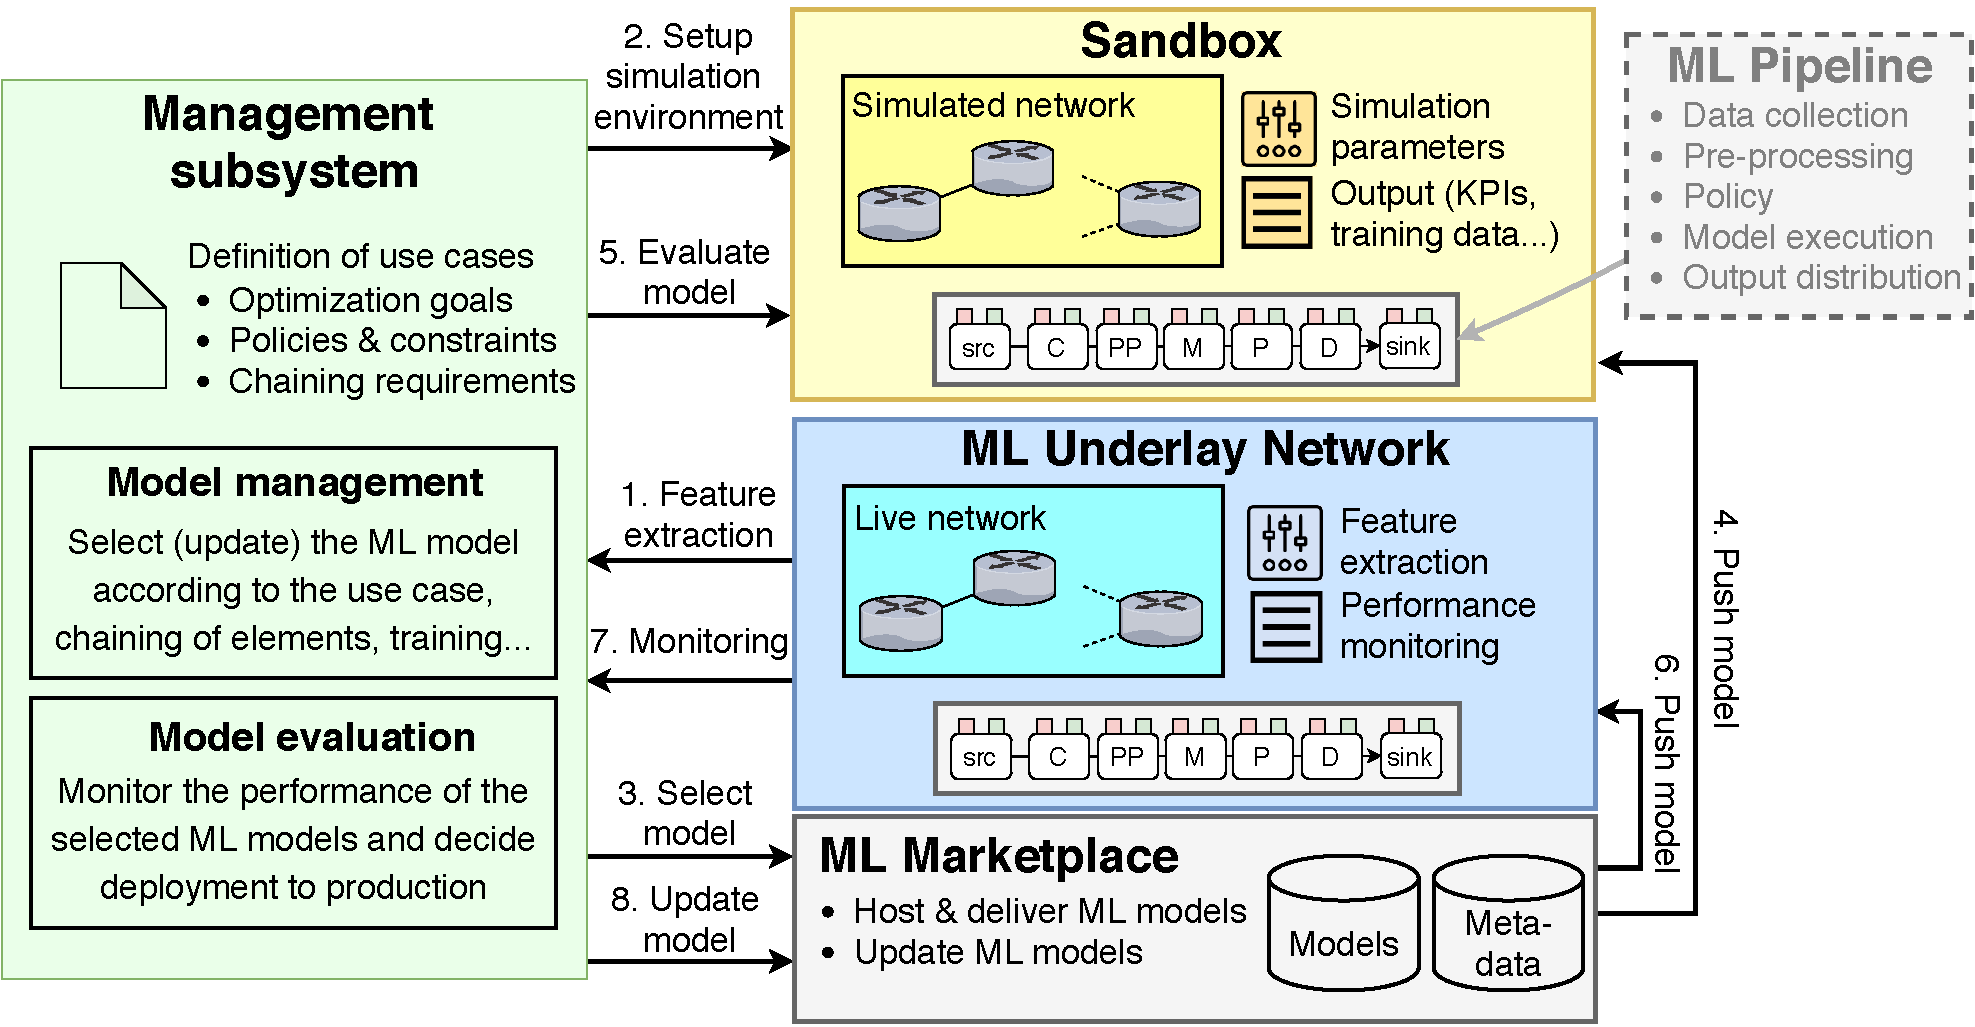
\includegraphics[width=0.7\textwidth]{architecture_example.pdf}
		\caption{Architectural elements and procedures for evaluating the output of ML models.}
		\label{fig:example_simulator}
	\end{figure*}
		
	\section{Network Simulators to Enable Artificial Intelligence in Communications}	
	In this Section, we describe the architectural aspects of integrating network simulators to ML-assisted communications. Besides, we analyze the key features and requirements for simulators to be included in an ML-based networking architecture.
	
	\subsection{Architectural Integration}
	Most of the existing simulation platforms have no relation with AI/ML techniques, nor have any integrated module for evaluating and training ML models. Moreover, current simulated network functionalities are typically too specific (e.g., simulate the effect of multiple antennas on the PHY layer performance), and seldom support open interfaces, as a result of being developed by focused academic or industrial organizations. To enable the next generation of ML-based communication systems, it is imperative to design interoperable mechanisms for simulated networks and ML mechanisms. For that purpose, we find of high relevance the ITU ML architecture defined in \cite{ITU3172}.	
	
    The ITU ML architecture defines a set of logical components, interfaces, and procedures to realize ML-assisted communications. For a complete overview of ITU architecture, we refer the interested reader to the work in \cite{itu_architecture}, which proposes a realization for future IEEE 802.11 WLANs, an important part of the 5G/6G ecosystem in unlicensed bands. In particular, the ML-aware architecture is composed of the following elements:
	\begin{itemize}
		\item \textbf{Management subsystem:} this element is responsible for the management and orchestration of the ML operation in a network. The responsibilities of this module range from data collection to model deployment and monitoring.
		\item \textbf{ML underlay network:} network at which the ML optimization is applied.
		\item \textbf{Sandbox:} evaluation domain that includes the usage of network simulators.
		\item \textbf{ML marketplace:} container of ML models that are applied to the ML underlay networks.
		\item \textbf{ML pipeline:} set of elements that interact with underlay networks to perform the ML optimization. 
	\end{itemize} 
	
	To integrate simulators in the loop of ML-assisted networks, standardization of elements, interfaces, and data handling procedures is key. This is captured by ITU architecture through the sandbox subsystem. The sandbox is an isolated domain for reproducing the behavior and operation of live networking systems, which is useful to evaluate the performance of ML models before being deployed in production environments. Network simulators can be included in the sandbox and used to evaluate and train ML models. To that end, interoperability allows building end-to-end ML pipelines in simulated network underlays.
	
	To illustrate the integration of network simulators within the high-level ITU architecture, Fig. \ref{fig:example_simulator} depicts an example where the output of an ML model is evaluated at the sandbox before being applied to the operative network. The involved procedures are as follows:
	\begin{enumerate}
		\item The management subsystem extracts features from the ML underlay network.
		\item Based on the characteristics of the ML underlay network, the simulation environment is prepared.
		\item The management subsystem selects the ML model from the marketplace, according to the meta-data describing the use case, the optimization goals, and the available ML models.
		\item The ML model is pushed to the sandbox to be applied to the simulated network.
		\item The ML model is evaluated in the simulator. Evaluation of other ML models may be considered upon unsuccessful results.
		\item Once the evaluation is successfully done, the ML model is pushed to the operative network, where the ML optimization takes place. 
		\item The network performance is monitored, as well as new data is gathered.
		\item The information obtained from monitoring is used to update the ML models and/or metadata in the marketplace.  
	\end{enumerate}

    The ML output evaluation procedure allows devising the potential benefits and drawbacks of using a certain ML-based optimization in a network. The fact is that ML outputs can sometimes look surprising from the perspective of a network operator, and their effect on the network may be unknown a priori. This is accentuated in complex problems for which ML is entailed to outperform legacy solutions because the knowledge on the problem is limited.

	\subsection{Practical Integration Aspects}
	
	To simulate multiple types of scenarios, technologies, and network functionalities, we find a plethora of proprietary and open-source network simulators (e.g., ns-3, OMNET++, OPNET, NetSim, Komondor). Apart from network technologies, we must take into account the capability of the different simulators to capture other specific phenomena in detail when required. This is the case, for instance, of Simulation of Urban MObility (SUMO) and UnderWater simulator (UWsim), which simulate vehicular urban mobility and underwater physical effects, respectively, and can be used along with OPNET and ns-3 simulators.
	     
	When it comes to integrating simulators into ML-assisted networks, a set of challenges arise with respect to execution, interoperability, and portability aspects:
	\begin{enumerate}
	    \item \textbf{Execution:} to test, train, and evaluate the performance of ML methods in simulators, it is important to reproduce the behavior of the target operative network. For the proper integration of simulators into the ML-aware architecture, it is required to transfer simulation-related meta-data to the elements of the ML pipeline. This includes supported technologies and network functionalities, maturity of simulation blocks (e.g., beta release), and the potential number of domains the simulators can span (e.g., from core to access network).
	            
	    Concerning pluggable ML functionalities, built-in ML modules can boost the procedures for simulating the behavior of ML mechanisms or training ML models in the sandbox. A few existing simulators support ML functionalities, but we find the framework connecting ns-3 with OpenAI Gym \cite{gawlowicz2019ns}, and the agent-based implementation in Komondor.
	    
        Apart from supported capabilities, short execution and configuration times can serve to empower ML-driven real-time applications. First, we consider the time it takes for the simulator to generate a given output, which may indicate the tractability of simulating large-scale scenarios. Second, fast reconfiguration of network simulators would allow following potential changes on the operative network (e.g., user demands, available resources, policies, etc.). For instance, an update of policies should be reflected in the simulation domain, so that operators' requirements can be fulfilled. 
        
        \item \textbf{Interoperability:} an important requirement lies in the degree of flexibility of simulators for interacting with the components of the ML-aware architecture. Interoperability is therefore meant to enable a seamless integration of intelligent network functionalities in the communication network. For that, it is imperative that the simulated network functionalities are managed using the same operation and maintenance mechanisms as for the network functionalities in the ML underlay. This can be achieved through standard Application Programming Interfaces (APIs). Features that may facilitate the interoperability of out-of-the-box simulators are the support for Command-Line Interface (CLI) execution mode, the level of monitoring supported (real-time, batch, model-based, etc.), and automation of data collection and in applying the ML output in the simulator (e.g., reading from log files vs. API-based interface with ML functions).

        \item \textbf{Portability:} network simulators are written in multiple programming languages (e.g., C/C++, Java) and supported by different specific platforms. Thus, portability is another important requirement for simulators. In this regard, containerization (e.g., via Docker) can be of great utility and allow network operators to deploy simulators in a flexible manner. Apart from that, parallelization is important to determine, for instance, the number of ML pipeline nodes and simulated network functionalities that the simulator can support at any instant.
    \end{enumerate}

	\subsection{Accuracy of Network Simulators}
	The degree of reliability of a network simulator depends on its accuracy on reproducing the actual real phenomena. In other words, simulations must be as close as possible to reality. This topic was previously addressed in \cite{accuracy_manet}, where the authors defended that simulators do not really fit the actual behavior of networks, based on experimental results in a MANETs testbed. Nevertheless, it was also shown that simulation results can serve as a good upper-bound for testbed setups.
		
	In general, network simulators accurately reproduce the behavior of protocols in higher levels of the TCP/IP stack. However, they can fail at characterizing complex physical phenomena such as radio propagation, antenna radiation, or energy consumption. As a result, network simulators typically provide accurate qualitative performance results and help to predict the behavior of real networks under certain circumstances. In contrast, results may lack quantitative precision, thus deviating from the exact performance that will be then experienced in real networking systems. Alternatively, hybrid approaches can be employed for simulating certain layers (e.g., MAC) while taking advantage of the actual interactions that occur in real implementations. Unfortunately, and to the best of our knowledge, there is little literature on this topic. 
		
	\section{Use-case: Power Control in Residential WLANs}	
	To illustrate the potential of integrating simulators to ML-assisted networks, we provide a testbed implementation of an IEEE 802.11 WLAN that suffers from starvation due to the high sensed interference of a residential environment. To address this problem, a joint ML-based solution is simulated and then provided to the testbed devices.
	
	\subsection{From Testbed to Simulation Domain}
	The considered testbed implementation comprises two overlapping Basic Service Sets (BSSs) in a residential environment, which are characterized by being highly dense and uncoordinated. The decentralized nature of WLAN deployments in a neighborhood may lead to high interference, which can be extremely variable due to the heterogeneous usage of the network and the complex physical phenomena that can occur. The non-stationarity of residential environments is, therefore, one of the critical aspects to be considered when designing dynamic solutions for improving network performance. Hence, the usage of network simulators can contribute to reducing the performance losses originated by transitory phases (e.g., exploration in online learning). 

	Our proposed testbed-simulator integration is illustrated in Fig. \ref{fig:testbed}, where the ML solution is provided by a simulated version of the testbed. Two identical BSSs are deployed in a high-density residential scenario. However, since they are positioned at different locations, they are subject to different interference conditions, and so offer different performance. The characterization of the WLAN testbed is done with the IEEE 802.11ax-oriented Komondor simulator, which includes the operation of agents for simulating the behavior of ML mechanisms when plugged into wireless nodes.\footnote{All the details of the experimental part and source code are open and available at the following repository: \url{https://github.com/fwilhelmi/usage_of_simulators_in_future_networks}, accessed on May 15, 2020.}
		
	\begin{figure}[ht!]
		\centering
		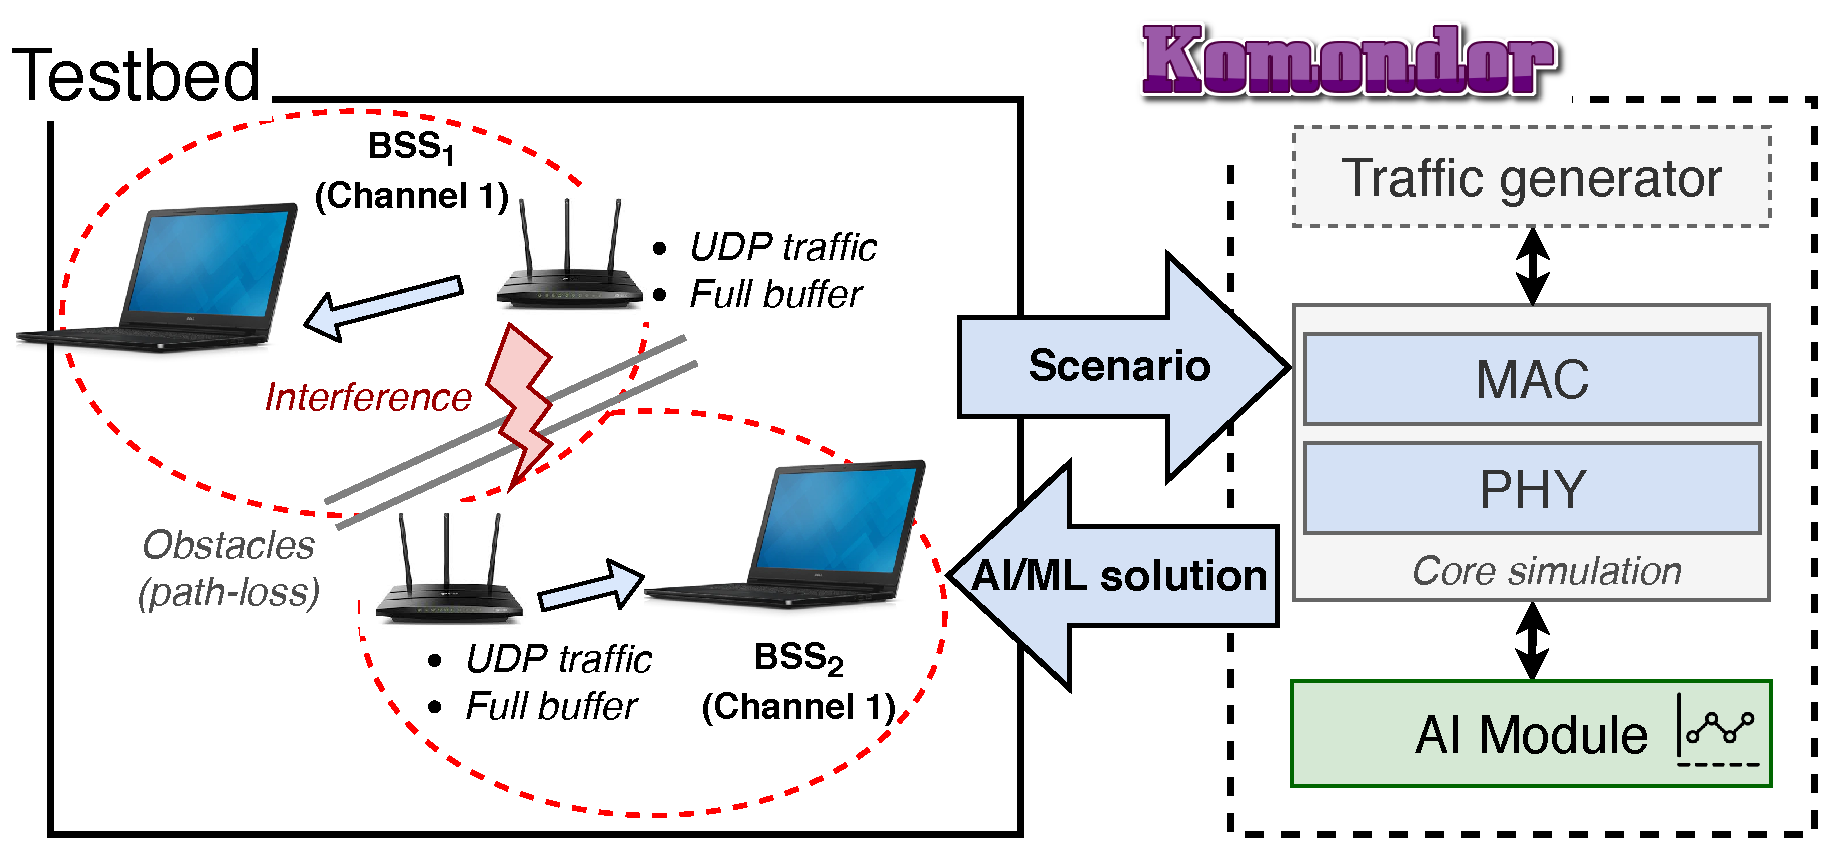
\includegraphics[width=\columnwidth]{testbed2.pdf}
		\caption{Use case application of the Komondor simulator to apply ML in a testbed WLAN.}
		\label{fig:testbed}
	\end{figure}

	Through the procedures that have been previously illustrated in Fig. \ref{fig:example_simulator}, the testbed scenario is first characterized in the simulator by gathering parameters such as the location of nodes, path-loss effects, or the traffic load. As an example of the characterization of the testbed in the simulator, consider the path-loss model selected, which is chosen based on the degree of similarity with respect to testbed measurements. After preparing the simulation environment, the ML model is applied in the simulator for the sake of improving a certain performance metric. Finally, the optimized ML-based configuration is passed and applied to the real devices, in which performance is expected to be enhanced.
	
	\subsection{Machine-Learning-based Transmit Power Control}
	To improve the performance of the target WLAN, we simulate a Multi-Armed Bandits (MABs) application for Transmit Power Control (TPC), as previously done in \cite{wilhelmi}. We take an online learning approach to address the complexity of spatial interactions in WLANs, where the effect of tuning the transmit power can be hindered. Accordingly, the MABs framework is useful to reduce the complexity of the problem and effectively improving the performance at a low computational cost. 
	
	This use case is particularly revealing since the transmit power is a critical parameter to be freely adjusted, and trying several configurations before finding the best performance may lead to unpredictable effects during the transitory regime. Moreover, commercial equipment typically offers a high delay when changing the transmit power or other parameters such as the primary channel. As a result, network simulators can play a crucial role in palliating the negative impact that exploration can have in communications.
	
	Figure \ref{fig:results_komondor} illustrates the temporal throughput obtained by each BSS when simulating the MABs approach for tuning the transmit power. Also, the performance that would be obtained by both BSS when using the default configuration is illustrated. As shown, both BSSs experience an unstable transitory regime before reaching a stable state whereby performance is improved. Among a set of input transmit power levels, the most popular one to be used by both BSSs is 7 dBm, which, based on simulation results, is expected to improve the average throughput by 88.48\%.
	
	\begin{figure}[ht!]
	\centering
	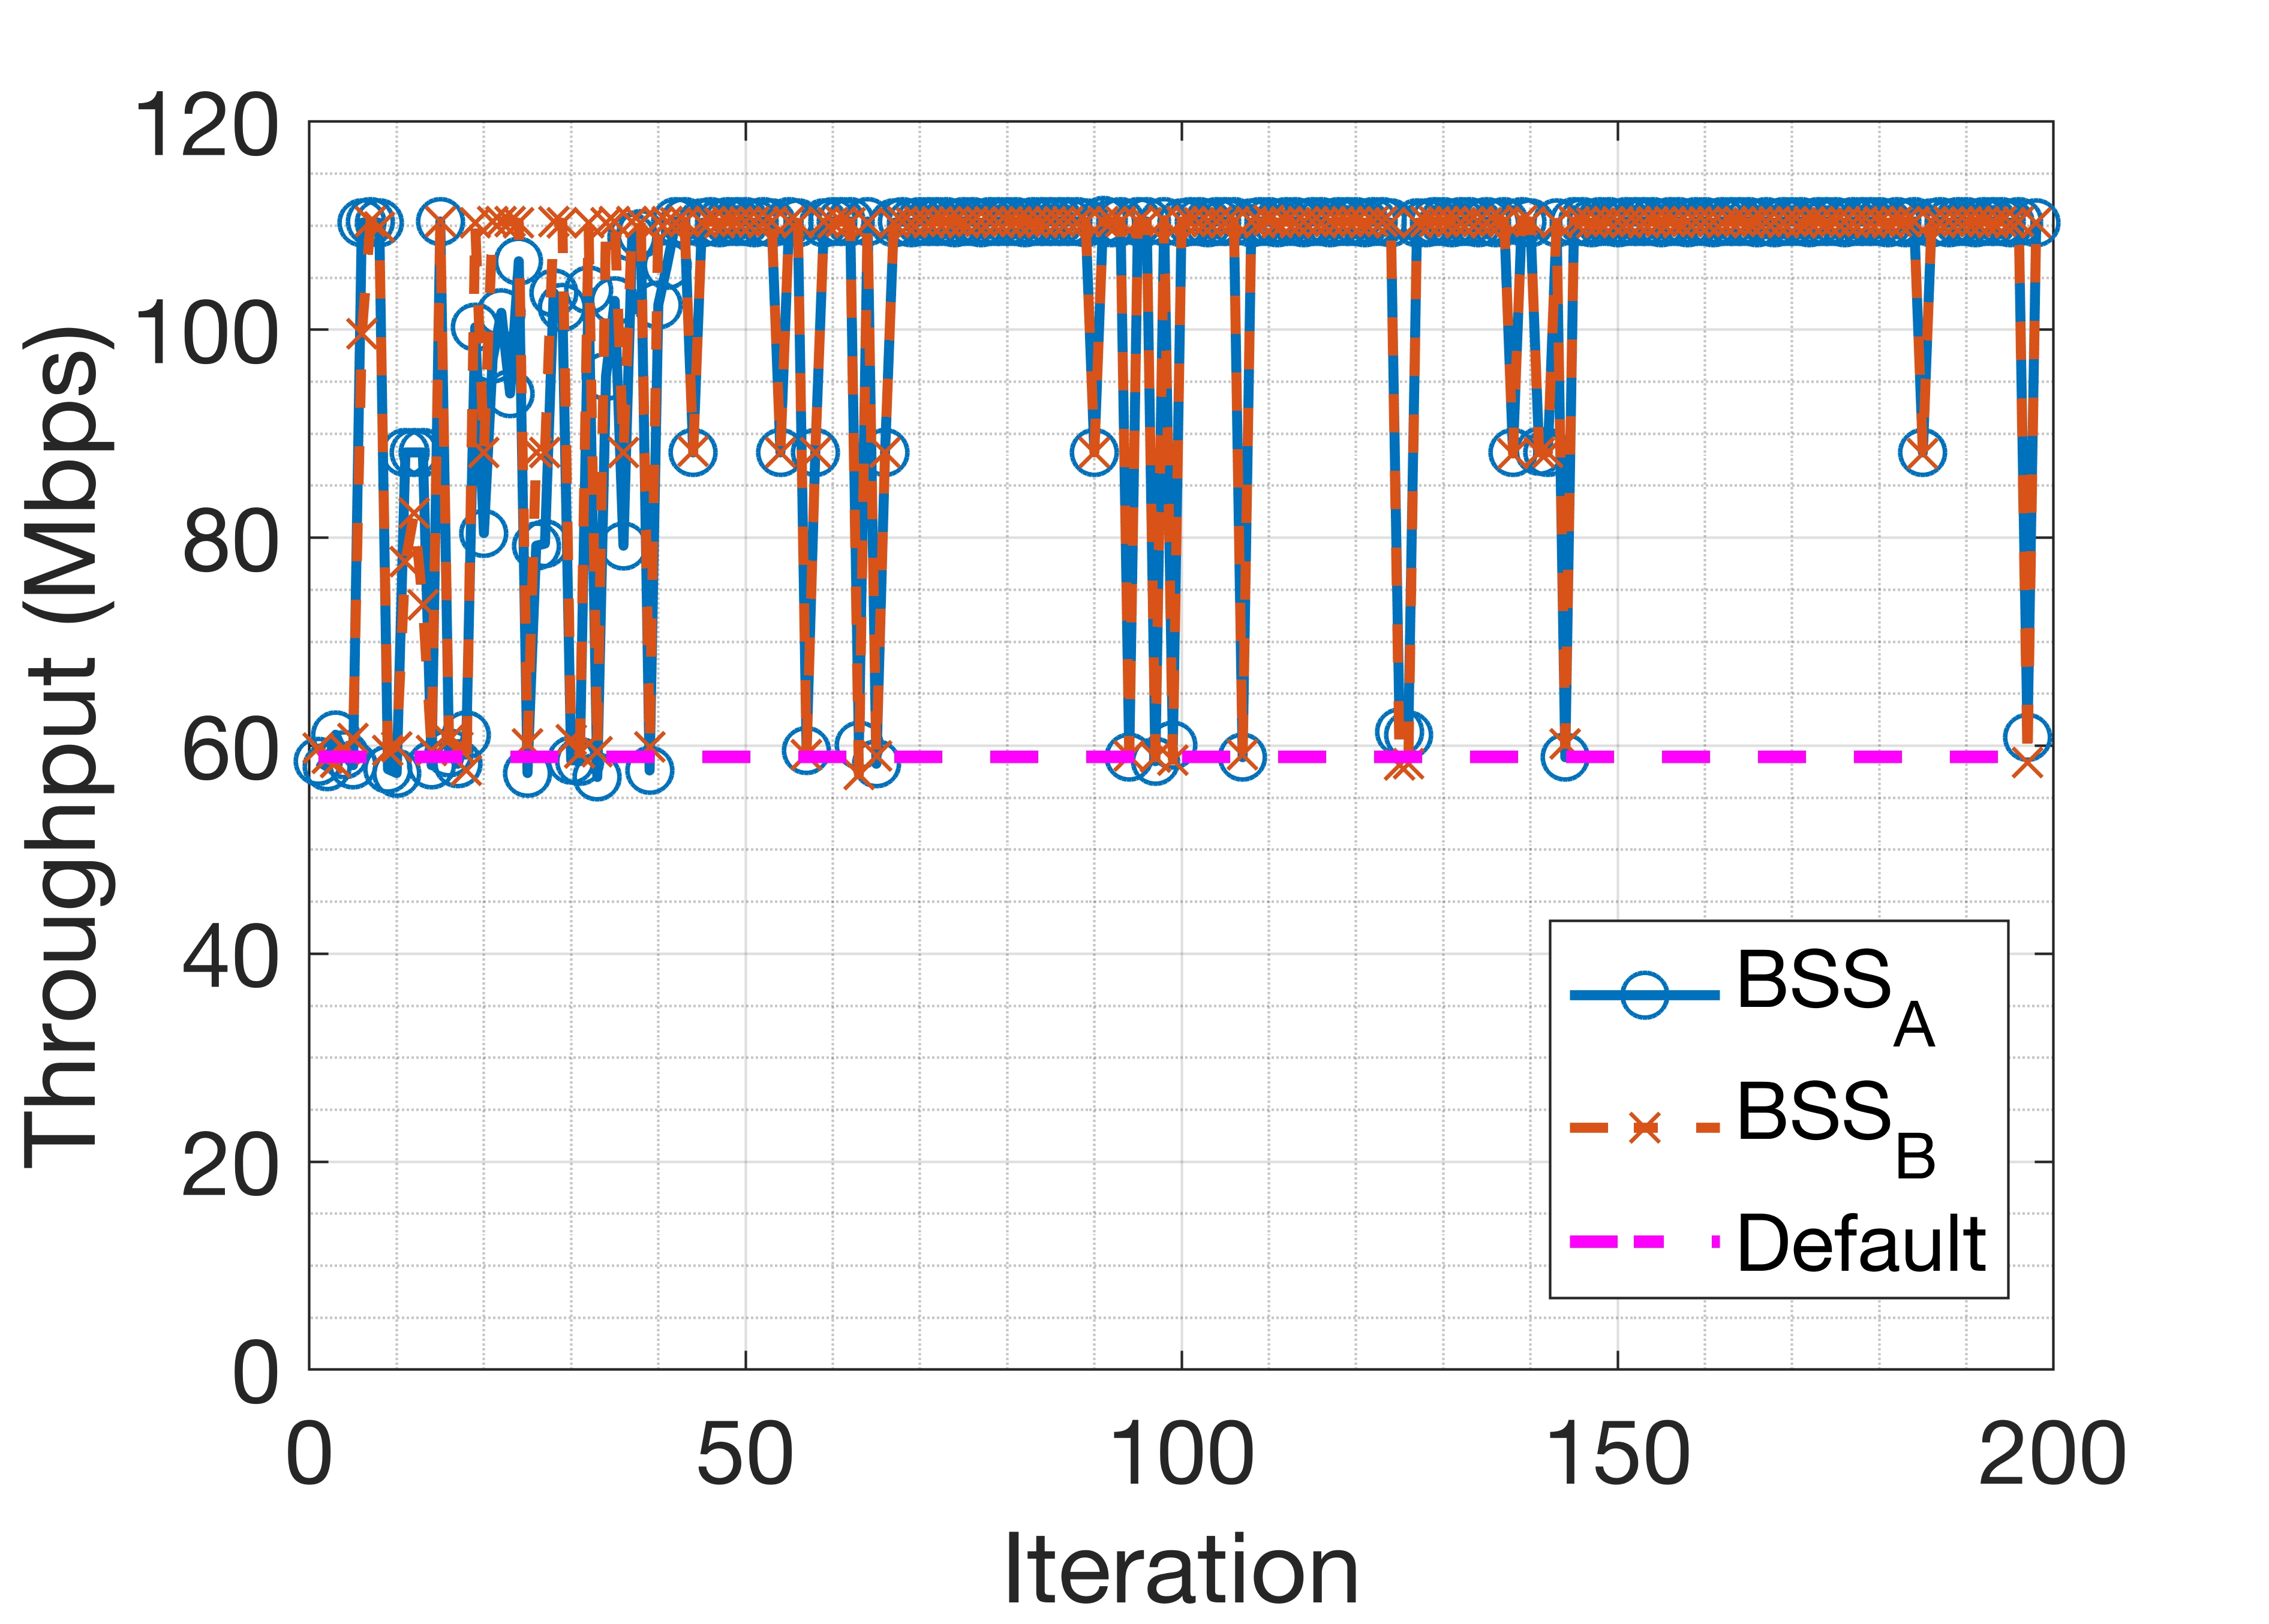
\includegraphics[width=0.8\columnwidth]{throughput_evolution_komondor.png}
	\caption{Simulated throughput evolution after applying MABs for tuning the transmit power in an OBSS. Each learning iteration corresponds to 5 seconds in the simulation.}
	\label{fig:results_komondor}
	\end{figure}
	
	Finally, we give some insights on the time it takes the simulator to bring up results for the testbed. To include the operation of simulators in future networks (especially for real-time applications), it is very important to find an equilibrium between the stability of the output and the time it takes to generate it. Figure \ref{fig:test_sim_time_vs_accuracy} shows the variability obtained on the simulation results, for different simulation time values. The execution time is also displayed. As observed, the higher the simulation time, the higher the stability is. However, this is paid with execution time, which varies for different network simulators. 
	
	\begin{figure}[ht!]
		\centering
		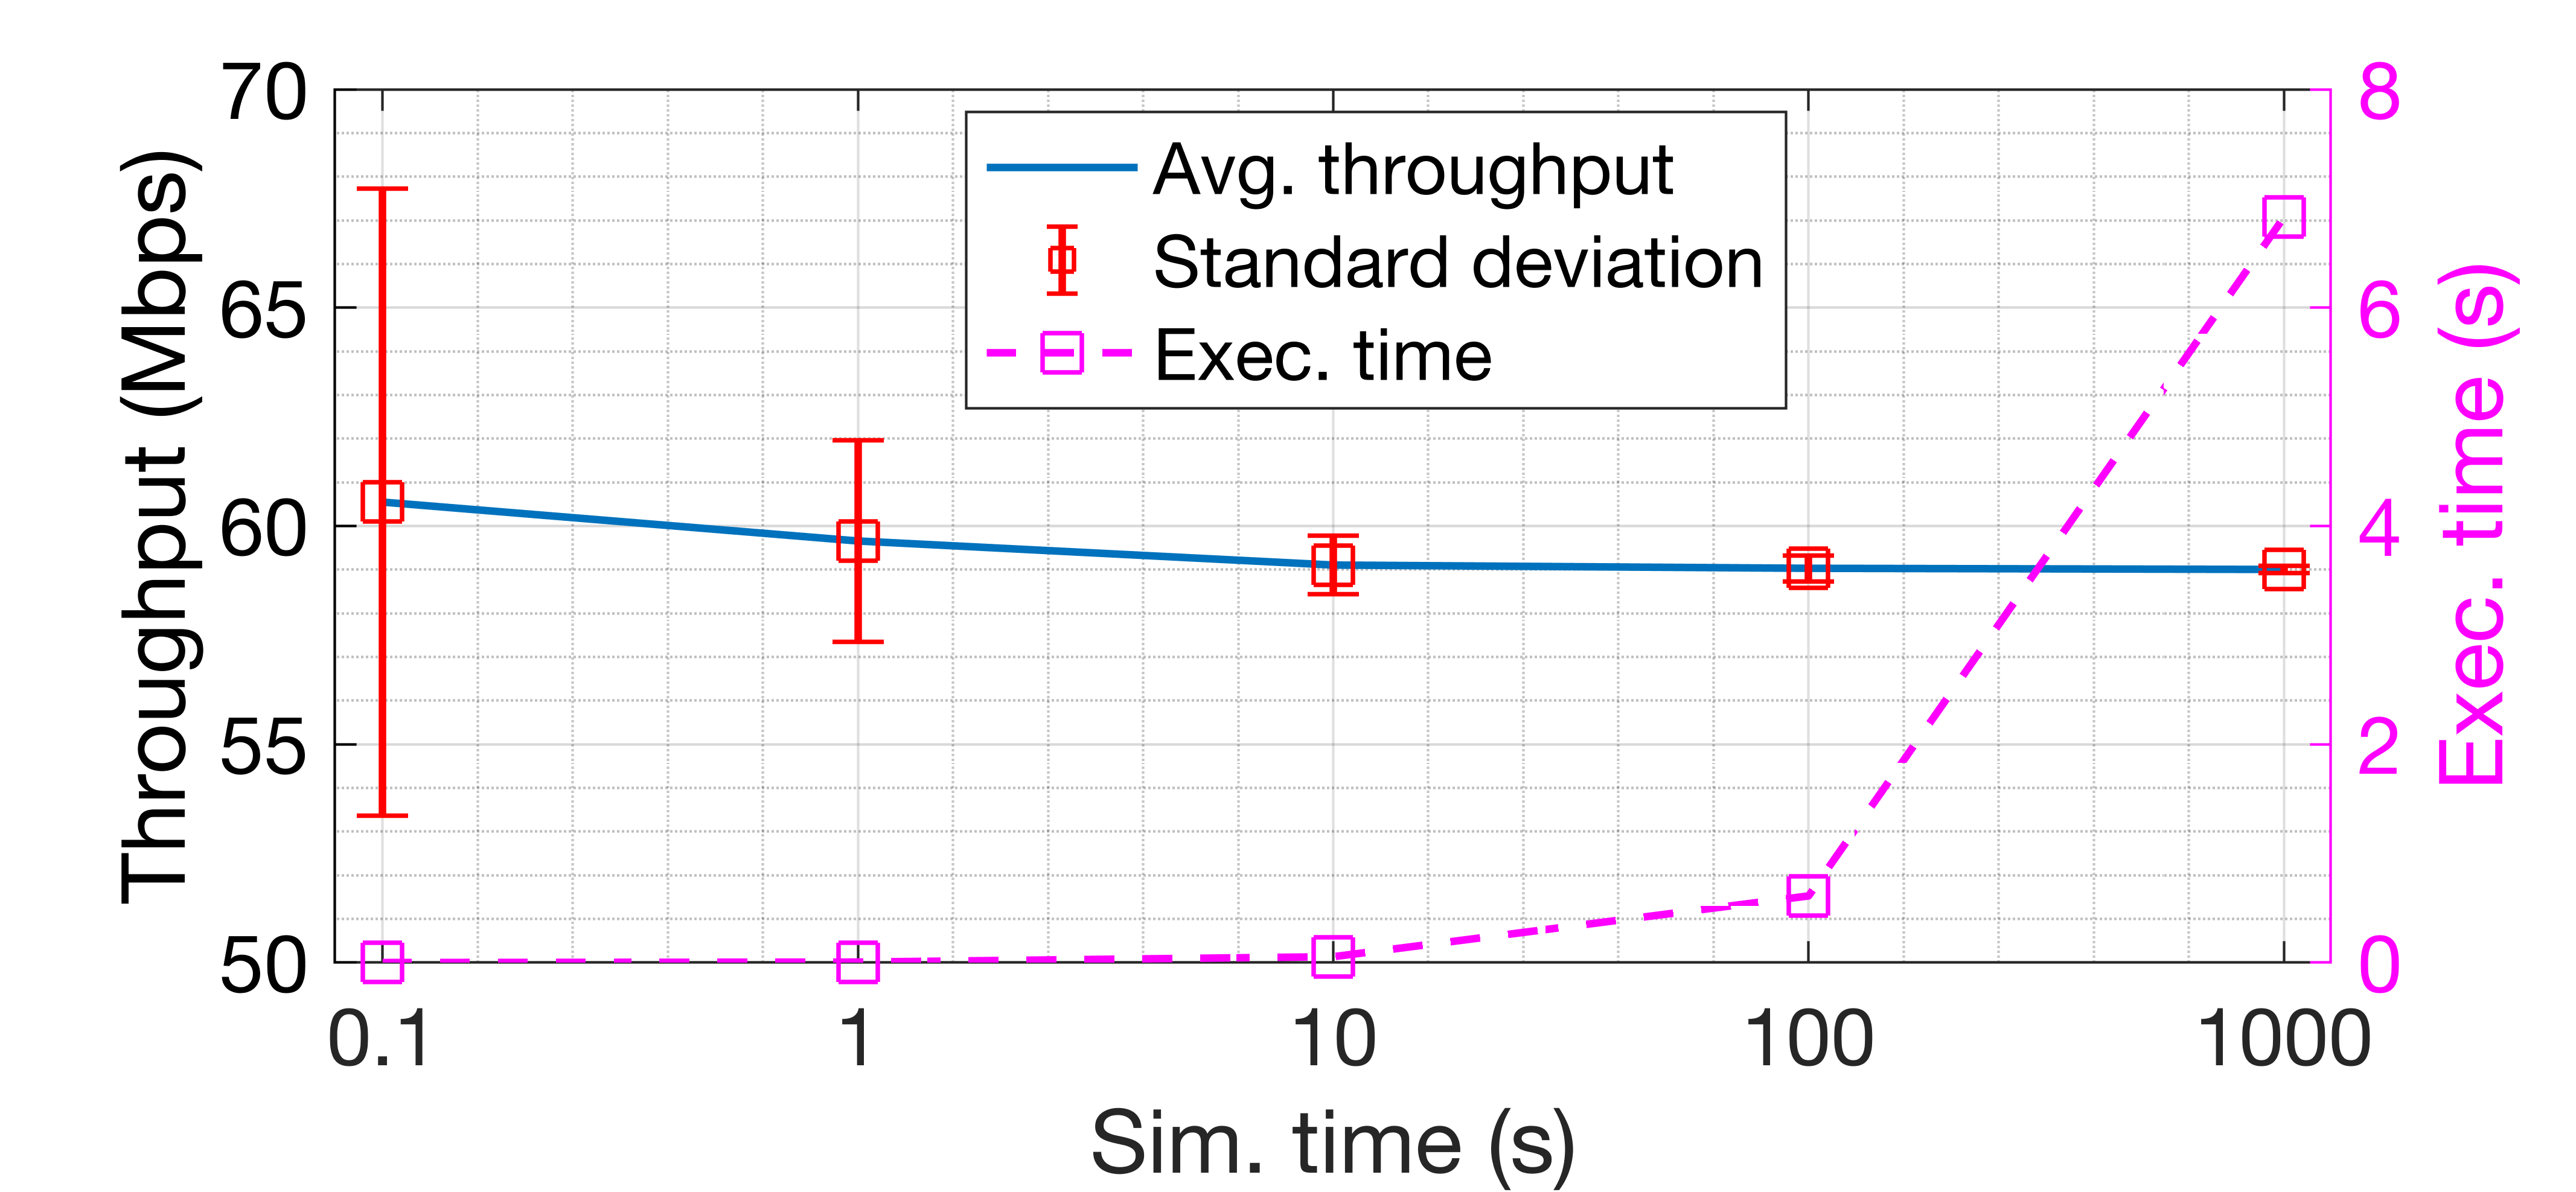
\includegraphics[width=0.9\columnwidth]{test_sim_time_vs_accuracy.png}
		\caption{Execution time versus variability of the results in Komondor simulator.}
		\label{fig:test_sim_time_vs_accuracy}
	\end{figure}

	\subsection{Testbed results}
	Now, we show the results of applying the configuration suggested by the simulator on the testbed. Figure \ref{fig:results} compares the performance of applying the ML-based configuration (both BSSs use a transmit power equal to 7 dBm) with that used by default (i.e., 23 dBm).
	
	As shown, both BSSs improve their throughput significantly by using the configuration suggested by the simulator. While BSS$_1$ improves its throughput by 76.16 \%, BSS$_2$ experiences a 93.98 \% improvement. Besides, based on the lower number of observed outliers, we notice higher stability in terms of throughput variability (especially for BSS$_1$). Note, as well, that BSS$_2$ suffers drops for some throughput values, which are originated by the high channel variability found at the residential environment the tests were performed.
	\begin{figure}[ht!!!!]
		\centering
		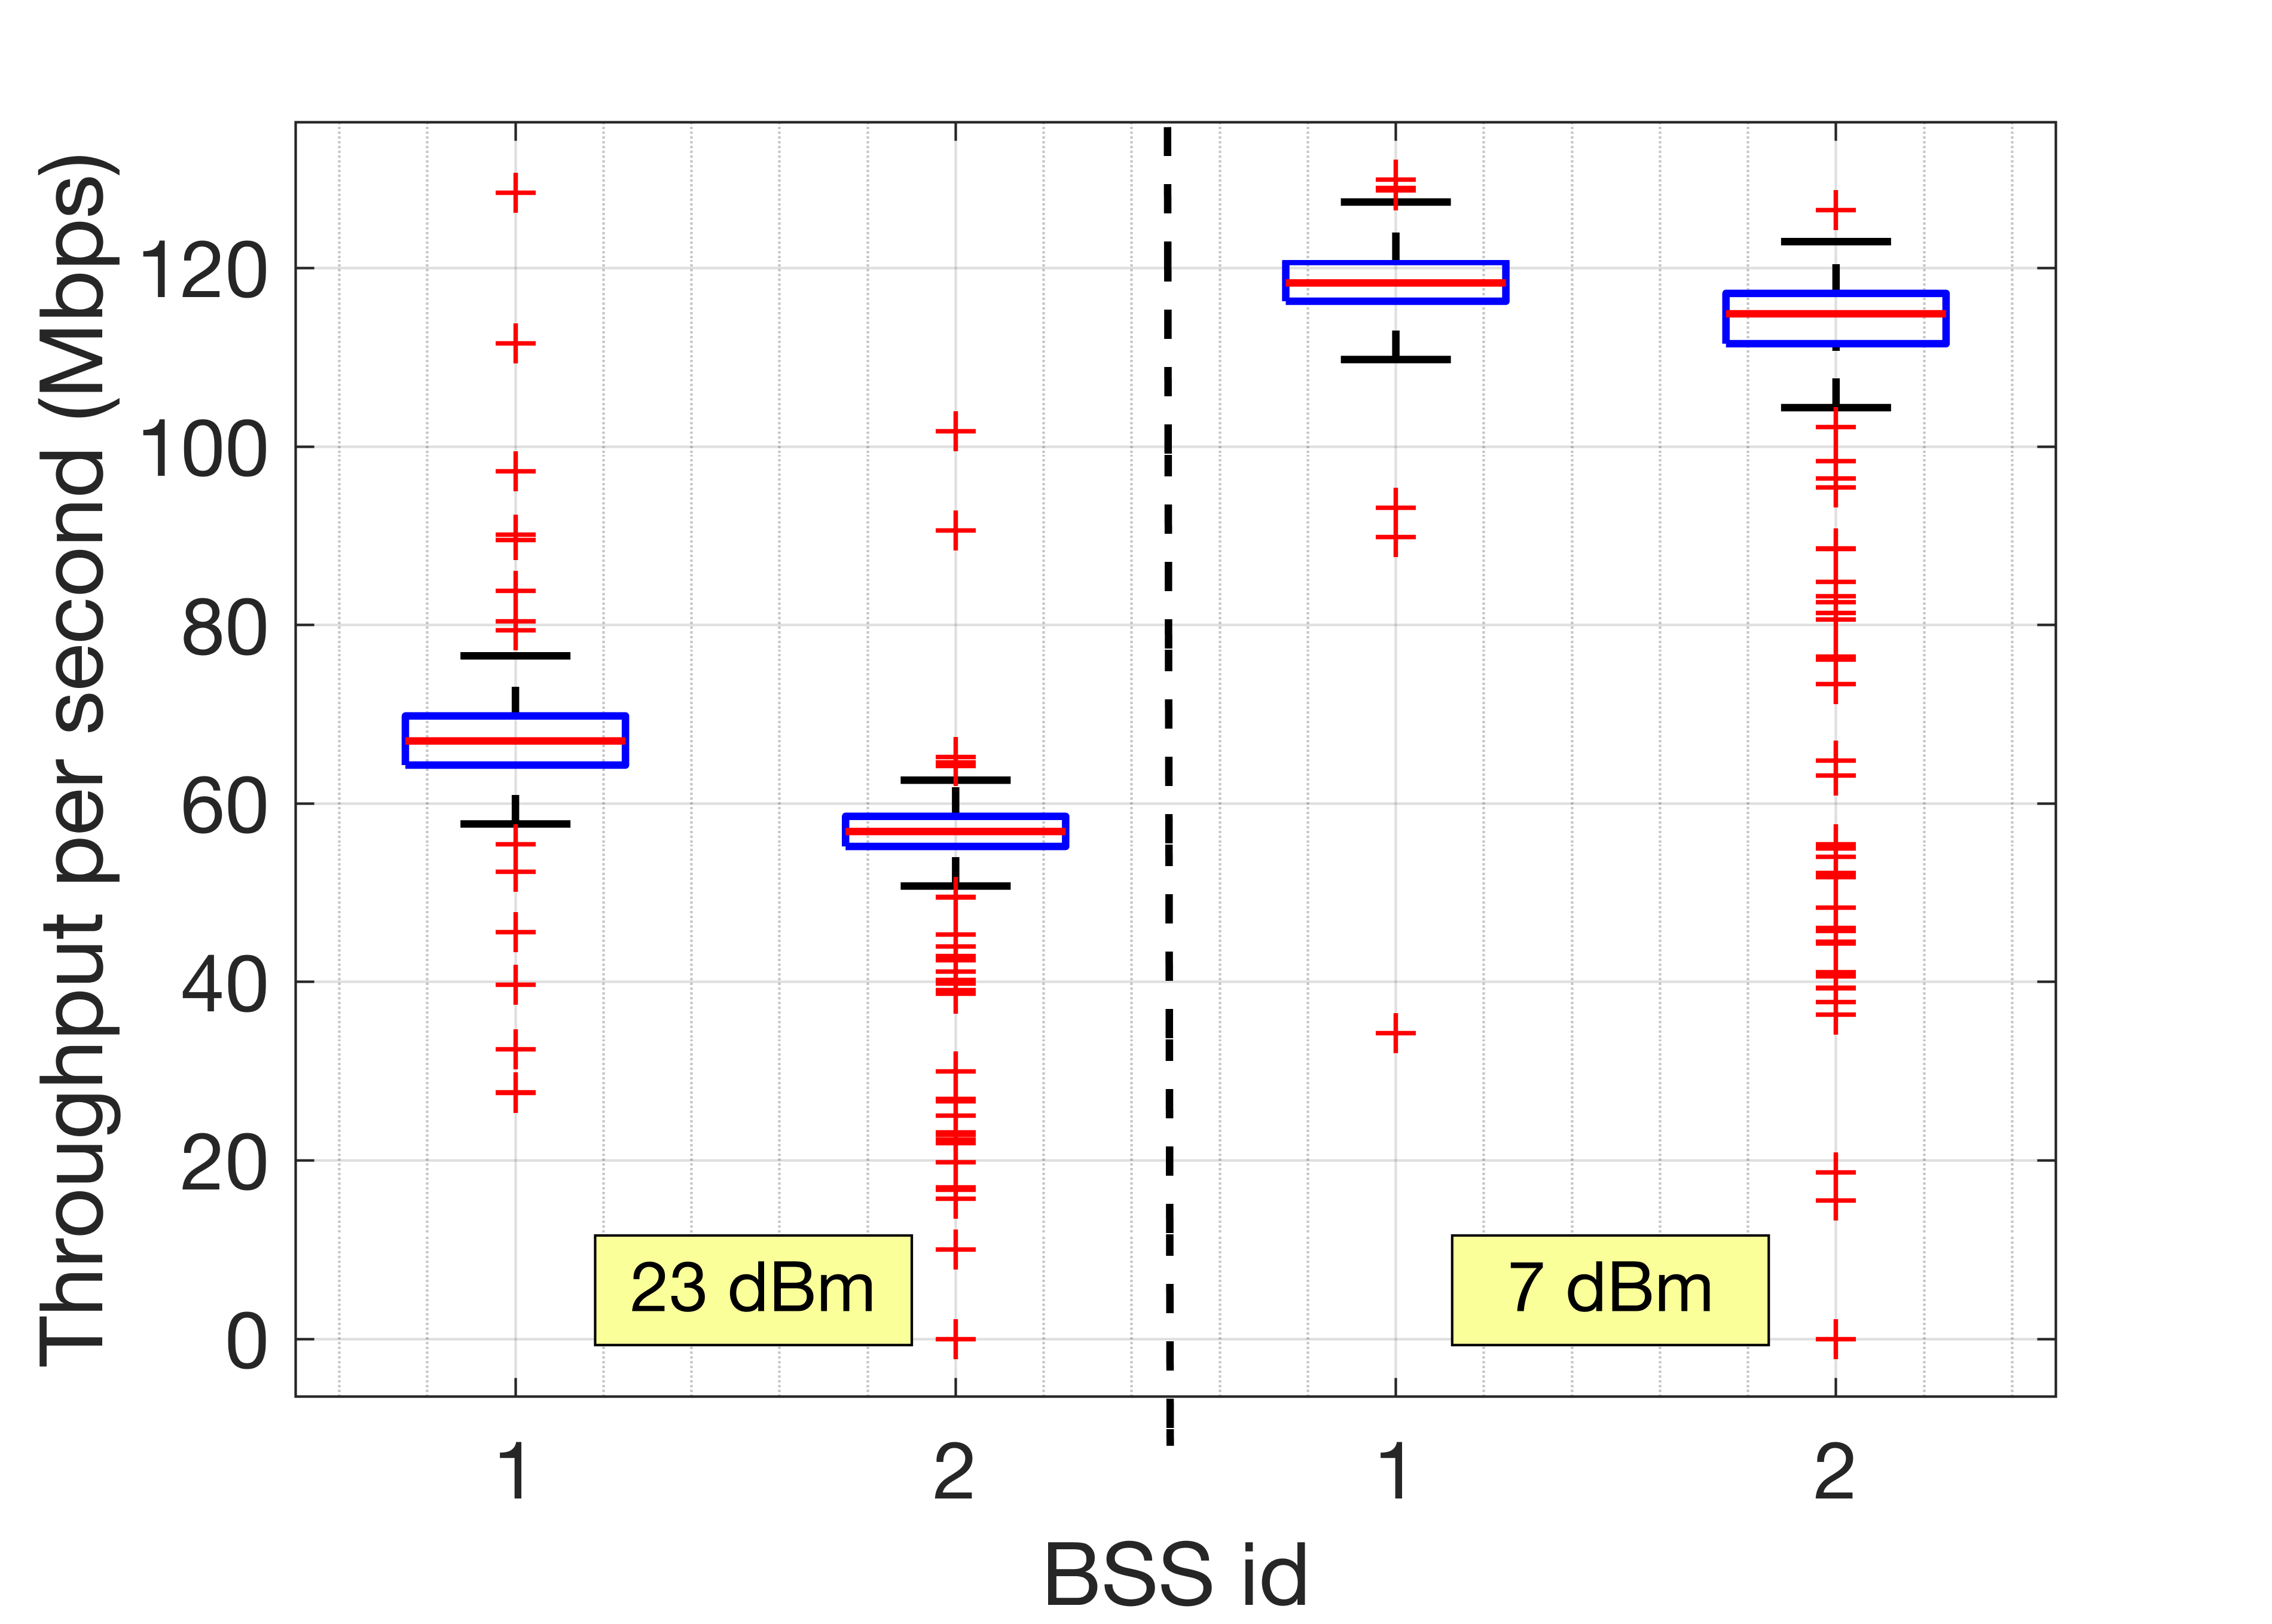
\includegraphics[width=0.8\columnwidth]{boxplotbps.png}
		\caption{Performance comparison of default (23 dBm) and ML-based (7 dBm) configurations at the testbed WLAN.}
		\label{fig:results}
	\end{figure}
	
	\section{Concluding Remarks}
	Future communications are expected to evolve towards automated systems enabled by ML. However, the application of ML to networking systems can generate instability and degrade KPIs. To address that, we envision the integration of sandbox environments for ML-assisted networks. In particular, we find network simulators of great utility for training, testing, and evaluating the performance of ML models before being deployed to production environments. In this article, we devised the potential usage of network simulators for future ML-based communications and provided insights on integration aspects. Our testbed results in a residential IEEE 802.11 WLAN showed how network simulators allow mitigating the negative effects of directly applying ML in the operative network.
	
	Network simulators are expected to contribute to filling the gap between AI and communications. Nevertheless, a lot of effort is still needed with regards to the architectural integration of simulators into ML-assisted networks. The most important challenges lie in the definition and implementation of standardized interfaces.

	\section*{Acknowledgment}
	This work has been partially supported by grants MDM-2015-0502, WINDMAL PGC2018-099959-B-I00 (MCIU/AEI/FEDER,UE), 2017-SGR-11888, and by SPOTS project (RTI2018-095438-A-I00) funded by the Spanish Ministry of Science, Innovation and Universities.
	
	\ifCLASSOPTIONcaptionsoff
	\newpage
	\fi
	
	\bibliographystyle{IEEEtran}
	\bibliography{bibliography}
	% if you will not have a photo at all:
	\begin{IEEEbiographynophoto}{Francesc Wilhelmi}
		(francisco.wilhelmi@upf.edu) holds a B.Sc. degree in Telematics Engineering (2015) and an M.Sc. in Intelligent and Interactive Systems (2016), both from Universitat Pompeu Fabra (UPF). He is currently pursuing a Ph.D. in Information and Communication Technologies at UPF.
	\end{IEEEbiographynophoto}
	%
	\begin{IEEEbiographynophoto}{Marc Carrascosa}
		(marc.carrascosa@upf.edu) obtained his B.Sc. degree in Telematics Engineering (2018) and a M.Sc. in Intelligent and Interactive Systems (2019) from Universitat Pompeu Fabra (UPF). He is currently a PhD student in the Wireless Networking Research Group in the Department of Information and Communication Technologies (DTIC) at UPF. His research interests are related to performance optimization in wireless networks.
	\end{IEEEbiographynophoto}
	%
	\begin{IEEEbiographynophoto}{Cristina Cano}
		(ccanobs@uoc.edu) holds a Ph.D. (2011) in Information, Communication and Audiovisual Media Technologies from Universitat Pompeu Fabra (UPF). She has been a research fellow in the Hamilton Institute of the National University of Ireland, Maynooth (2012-2014), in Trinity College Dublin (2015-2016) and in Inria-Lille in France (first half of 2016). Currently, she is an associate professor at Universitat Oberta de Catalunya (UOC). 
	\end{IEEEbiographynophoto}
	%
	\begin{IEEEbiographynophoto}{Anders Jonsson} (anders.jonsson@upf.edu) is the director of the Artificial Intelligence and Machine Learning group at Universitat Pompeu Fabra (UPF). He received his Ph.D. in computer science in 2005 from the University of Massachusetts Amherst, USA, and has been at UPF ever since.
	\end{IEEEbiographynophoto}
	\begin{IEEEbiographynophoto}{Vishnu Ram}
	(vishnu.n@ieee.org) worked for Motorola/Nokia/Siemens in advanced technologies teams for 21 years. He was a Scientific Advisory Board Associate (SABA) member of Motorola Networks. He has published several drafts in IETF, contributed to ETSI, 3GPP in his role as a senior specialist (Radio Resource Management). He is currently working as an independent researcher.	
	\end{IEEEbiographynophoto}
	%
	\begin{IEEEbiographynophoto}{Boris Bellalta}
		(boris.bellalta@upf.edu) is an Associate Professor in the Department of Information and Communication Technologies (DTIC) at Universitat Pompeu Fabra (UPF). He is the head of the Wireless Networking research group at DTIC/UPF.
	\end{IEEEbiographynophoto}
	\vfill
	
\end{document}